\documentclass[a4paper,12pt]{article}
\usepackage{amsmath}
%\usepackage{polish}
\usepackage[polish]{babel}
\usepackage[utf8]{inputenc}
\usepackage[T1]{fontenc}
\usepackage{graphicx}
\usepackage{anysize}
\usepackage{enumerate}
\usepackage{times}
\usepackage{plain}
\usepackage{caption}
\usepackage{graphicx}
\usepackage{setspace}
\usepackage{multirow}
\usepackage{lipsum}
\usepackage{indentfirst}
%\marginsize{left}{right}{top}{bottom}
\marginsize{2.5cm}{2.5cm}{2.5cm}{2.5cm}
\setlength{\parindent}{4em}
\setlength{\parskip}{1em}
\renewcommand{\baselinestretch}{2.0}



\begin{document}
\onehalfspacing

\begin{figure}[!htb]
	\centerline{
\includegraphics[scale=0.8]{agh_logo.jpg}}
\end{figure}

\begin{center}
	\Huge{Modelowanie i Symulacja Systemów\\
		Data-driven modelling:\\ Predykcja ruchu samochodów\\}
	\date{}
%	\maketitle

	\vspace{3cm}
	\Large{	Autorzy:\\
		Łukasz Gosek\\
		Fryderyk Muras\\
		Przemysław Michałek\\}

	\newpage

	
\end{center}
%\begin{enumerate}
%	\item \textbf{{\Large Wprowadzenie}}\\ \\
\section{Wprowadzenie}

%		\begin{large}
Zatory komunikacyjne przyciągają uwagę wielu naukowców, ponieważ stają się jednym z największych problemów środowisk miejskich. Coraz większa liczba samochodów codziennie przemierzających miejskie drogi w połączeniu z niedostosowaną do zapotrzebowania infrastrukturą powoduje niedogodności dla kierowców ale również dla wszystkich innych mieszkańców miast. Konieczne jest odpowiednie modernizowanie i tworzenie nowej infrastruktury drogowej, a to z kolei wymusza istnienie odpowiedniego aparatu do symulacji zjawiska ruchu miejskiego.
		
\section{Przegląd literatury}

Aby zrozumieć zjawisko zatłoczenia ruchu, naukowcy przeprowadzili wiele badań na podstawie różnych modeli i metod. Model automatu komórkowego (Cellular Automaton) opracowany przez Nagela i Schreckenberga \cite{nagel1992cellular} jest jednym z najwydajniejszych modeli problemów z przepływem ruchu.
Przepływ ruchu jest zależny od kilku czynników, w tym od zachowania kierowców (np. niedoskonały styl jazdy, wolniejsze samochody i wypadki), które odgrywają ważną rolę w tworzeniu się korków w systemie transportowym, zwłaszcza w połączeniu ze wzrostem ilości i co za tym idzie gęstości samochodów \cite{chowdhury2000statistical}. Gdy zwiększa się gęstość samochodów zachodzi przejście fazowe: ze swobodnego przepływu do fazy przeciążenia. W fazie swobodnego przepływu samochody poruszają się z prędkością bliską ograniczeniu, co prowadzi do zwiększenia gęstości pojazdów. Jednak faza przeciążenia charakteryzuje się ujemną liniową zależnością między przepływem ruchu a gęstością. Wykazano, że w fazie przeciążenia zachowanie kierowców ma znaczny wpływ na przestrzenną dystrybucję pojazdów na drodze
względem siebie \cite{jarai2012earthquake}.
Jednym z rozwiązań rozładowania zbyt gęstego ruchu drogowego jest rondo - skrzyżowanie bez świateł oferujące rozwiązania
korzystne pod względem bezpieczeństwa obiegu, opóźnień i przepustowości. Zostało po raz pierwszy opracowane w Wielkiej Brytanii i obecnie jest szeroko stosowane w
większości państw. Kierowcy zbliżający się do ronda muszą zmniejszyć prędkość i przed wjazdem szukać potencjalnych konfliktów z pojazdami, które już są na rondzie.

W wielu raportach stwierdzono, że ryzyko wypadku na rondach znacznie zmalało
w porównaniu z innymi konwencjonalnymi skrzyżowaniami \cite{persaud2001safety}. Jednak wypadki samochodowe na środku ronda są jednym z najczęstszych czynników przyczyniających się do powstawania zatoru. Wśród przyczyn wypadków samochodowych jest wysoka prędkość i wymuszanie pierwszeństwa. Pomimo wykazanych korzyści bezpieczeństwa rond, wypadki na nich zdarzają się regularnie. Badanie kolizji na 38 rondach w Maryland wykazało, że zdarzały się one częściej
przy wjazdach na ronda niż wewnątrz czy przy wyjściach \cite{mandavilli2009crash}.
%		\end{large}


%	\begin{enumerate}
%		\item a
%		\item b
%		\item c
%		\item d 
%	\end{enumerate}

%	\newpage
%	\item \textbf{{\Large Proponowany model}}\\ \\
%	 \begin{large}

\subsection*{Modele matematyczne}
			Wspomniane we wprowadzeniu automaty komórkowe można przedstawić w postaci czwórki (L, S, N, f), gdzie kolejne elementy oznaczają: przestrzeń podzieloną na siatkę cel, zbiór skończonych stanów, zbiór sąsiadów danej celi oraz funkcję zmiany konfiguracji w poszczególnych celach. Konfiguracja C:L $\rightarrow$ S jest funkcją, która łączy każdą celę siatki ze stanem. Funkcja f zmienia konfigurację C$_{t}$ w nową konfigurację C$_{t+1}$. O klasyfikacji automatów komórkowych można dowiedzieć się więcej w pracy \cite{wkasalgorytmy} o ich użyciu, również dla predykcji ruchu pieszych, w pracy \cite{wkas2004zastosowanie}, dokonano też w pracy \cite{dudek2005formalizacja} pewnej formalizacji dla automatów ze stałą siatką, wykorzystywanych do modelowania systemów o stałej topologii przestrzennej. Założenia tej pracy będą wykorzystywane w dalszej części projektu.
			
			 Klasycznym modelem opisującym ruch samochodowy (opartym na automatach komórkowych) jest model Nagela-Schreckenberga \cite{nagel1992cellular} (nazywany krócej \textit{Na-Sch}). Model ten z założenia opisuje ruch samochodów na autostradzie, lecz po kilku modyfikacjach można opisać nim również ruch miejski. W modelu \textit{Na-Sch} przyjęty został stały rozmiar komórki równy \textit{d = 7,5} m, w każdej komórce może znajdować się tylko jeden pojazd, prędkość pojazdu opisywana jest liczbą komórek pokonywanych przez pojazd w następnej iteracji. \textit{Na-Sch} opisują następujące reguły ruchu:
			 \begin{itemize}
				\item Przyspieszenie: \textit{v(t + 1)} $\rightarrow$ min( \textit{v(t} + 1), \textit{v}$_{max}$), gdzie \textit{v(t)}	to prędkość aktualna
				\item Hamowanie: \textit{v(t + 1)} $\rightarrow$ min( \textit{v(t} + 1), \textit{g(t)} - 1), gdzie \textit{g(t)}	jest liczbą pustych komórek pomiędzy pojazdami
				\item Element losowy (nieuzasadnione, przypadkowe hamowanie): prawdopodobieństwo \textit{p}, że nastąpi \textit{v(t} + 1) $\rightarrow$ max(\textit{v(t} - 1)), jeżeli \textit{v(t)} >= 1
				\item Ruch: \textit{x(t + 1)} = \textit{x(t)} + \textit{v(t)}
			 \end{itemize}
			
			\begin{figure}[!htb]
				\centering
				\captionsetup{justification=centering,margin=2cm}
				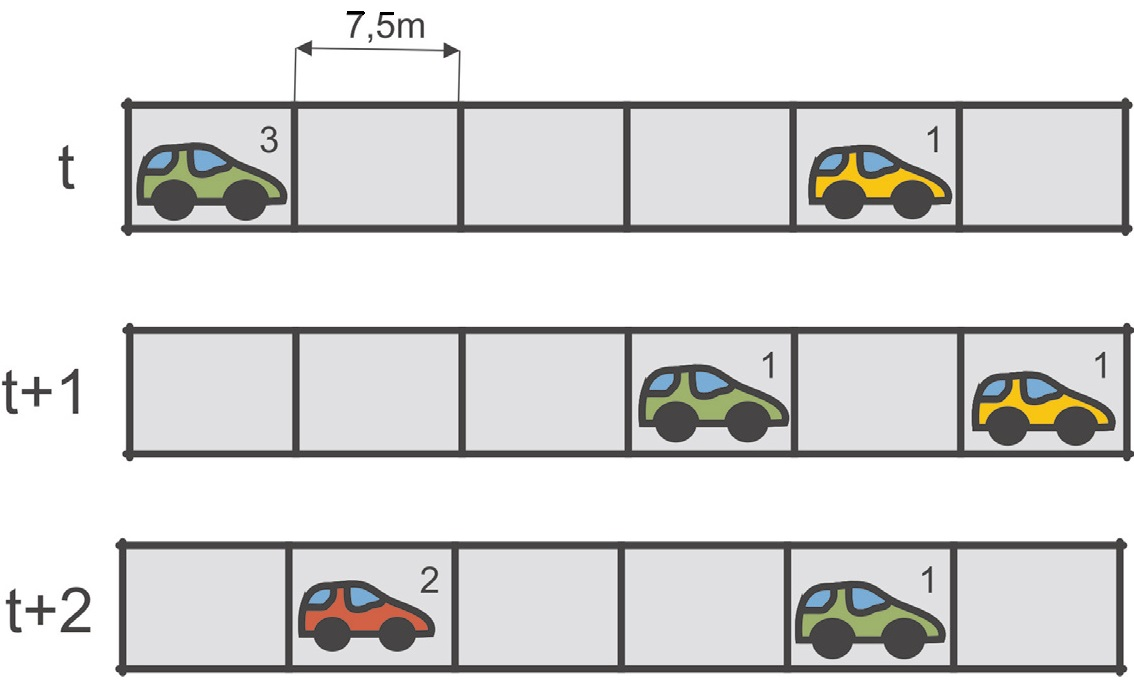
\includegraphics[scale=0.35]{Na-Sch.jpg}

				\caption{Ruch w \textit{Na-Sch} dla jednego pasa ruchu. \\Liczby przy samochodach oznaczają aktualną prędkość pojazdu $\rightarrow$ liczbę pokonywanych komórek w trakcie iteracji (źródło: \cite{WBGO2009})}
			\end{figure}
			
	\newpage			
			
			Na bazie modelu \textit{Na-Sch} stworzono z sukcesem szereg wiarygodnych modeli dla ruchu samochodowego o czym świadczy liczba łącznych cytowań (ponad 4 500) artykułu w którym model został opublikowany. Wśród tych prac należy wyróżnić pracę Hartmana \cite{hartman2004head} w której autor wprowadza nie tylko obsługę wielu pasów ruchu jak również ronda, skrzyżowania, uwzględnia długości poszczególnych typów pojazdów (motocykl, samochód, ciężarówka etc) oraz odpowiednio modyfikuje prędkości dla potrzeb realizmu modelu. Bardzo szczegółowo wykorzystanie \textit{Na-Sch} opisuje również praca \cite{regragui2018cellular} gdzie z kolei każde skrzyżowanie zastąpione jest rondem.
			
			Głównym powodem dla którego czysty model \textit{Na-Sch} nie gwarantowałby wiarygodnych rezultatów dla ruchu w mieście jest jego pierwotne założenie: ma opisywać ruch na autostradzie. Ruch pojazdów na autostradzie diametralnie różni się od ruchu miejskiego, gdzie pojazdy naprzemiennie przyspieszają i hamują. Niemal każdy samochód porusza się z inną prędkością niż jadący blisko inny pojazd co wymaga innego podejścia. Różnice pomiędzy modelowanym ruchem miejskim a rzeczywistością opisuje książka \cite{wagner1995traffic}.
			%////////////////////////////
%W naszym modelu wprowadzono odpowiednie modyfikacje:
%			\begin{itemize}
%				\item Przedwczesne unikanie kolizji: zwalnianie przed najbliższym  pojazdem z dużym wyprzedzeniem
%				\item Warunki koniecznie do zmiany pasa ruchu: zbliżanie się do poprzedzającego pojazdu oraz wolny pas obok
%				\item Szansa niezmienienia pasa ruchu pomimo spełnionego warunku zmiany (losowość zachowania kierowców)
%			\end{itemize}
%//////////////////////////////
%\end{large}
\newpage
\section{Proponowany model}
\label{sec:model}

Podstawą stosowanego przez nas modelu jest klasyczny model Nagela-Schreckenberga. Modyfikacji uległy:

\begin{itemize}
	\item długość komórki automatu - u nas $ 2,5 m$
	\item maksymalna prędkość samochodów  jest losowana z przedziału $[3;5]$. Ma to symulować różne typy pojazdów i różne profile psychologiczne kierowców poruszających się po drogach.
\end{itemize}

W dalszej kolejności, w oparciu o artykuł \cite{nagel1995twolane} model został rozszerzony na obsługę wielu pasów ruchu. Co do zasady jest to kilka automatów komórkowych implementujących model Na-Sch z dodanymi regułami przejścia pomiędzy tymi automatami. Samochód $i$ zmienia pas jeśli spełnione są następujące warunki:

\begin{subequations}
\label{eq:przejscia}
\begin{align}
gap(i) &< l \label{eq:przejscia1} \\
gap_{o}(i) &> l \label{eq:przejscia2} \\
gap_{o, back} &> l{o, back} \label{eq:przejscia3} \\
rand() &< p_{change} \label{eq:przejscia4}
\end{align}
\end{subequations}

Oznaczenia: $gap(i)$ - liczba wolnych komórek do samochodu poprzedzającego na tym samym pasie, $gap_{o}(i)$ - liczba wolnych komórek do najbliższego samochodu z przodu na docelowym pasie, $gap_{o,back}(i)$ - liczba wolnych komórek do najbliższego samochodu z z tyłu na docelowym pasie, $l, l_{o,back}$ - parametry oznaczające jak daleko ,,kierowca patrzy na sąsiednim pasie'' przy zmianie pasa, $p_{change}$ - prawdopodobieństwo zmiany pasa (symuluje nieracjonalne zachowanie kierowcy - pozostanie na aktualnym pasie mimo spełnionych przesłanek do jego zmiany). Dodatkowo przy zmianie pasa na bliższy prawej krawędzi jezdni nie stosuje się warunku \ref{eq:przejscia1}. Ma to na celu odwzorowanie wymuszonej przepisami ruchu drogowego jazdy możliwie blisko prawej krawędzi jezdni.

Kolejnym poziomem jest połączenie modeli wielopasowych w sieć dróg. W tym celu w automatach komórkowych modelujących pojedynczą drogę periodyczne warunki brzegowe zostały zastąpione zmodyfikowanymi warunkami pochłaniającymi - po wyjściu ,,poza drogę'' samochód, z pewnym rozkładem prawdopodobieństwa, przemieszcza się do którejś z innych dróg na danym skrzyżowaniu i tam kontynuuje swoją podróż. Na każdym ze skrzyżowań została zaimplementowana podstawowa wersja sygnalizacji świetlnej zapewniająca brak kolizji między pojazdami. Dodatkowo na każdym skrzyżowaniu zliczane są samochody, które przez nie przejechały (będą to dane analizowane po zakończonej symulacji).

Na brzegach modelowanego fragmentu sieci drogowej zaimplementowany jest mechanizm generowania nowych samochodów i usuwania tych, które opuszczają dany obszar.

Takie modele skrzyżowań i dróg, przy określeniu sposobu generowania samochodów (na przykład na podstawie danych pomiarowych) pozawalają na zamodelowanie fragmentu miasta i symulację ruchu samochodów wewnątrz niego. Generowanie samochodów może następować w oparciu o zewnętrzne dane zawierające informacje o natężeniu ruchu w określonych punktach. 
%\newpage
\section{Symulacja zjawiska}
\subsection*{Modelowany obszar}
Na potrzeby symulacji zamodelowany został fragment miasta Darmstadt położonego na południowym zachodzie Niemiec, na południe od Frankfurtu nad Menem. Darmstadt to niewielkie miasto, liczy około 150 tys. mieszkańców (stan na 2015 rok), w związku z czym natężenie ruchu miejskiego nie jest w nim zbyt duże, jednakże dostępne są dla niego bardzo dokładne dane o natężeniu ruchu. Przedsiębiorstwo ,,[ui!] Urban Software Institute GMBH''\footnote{https://www.ui.city/de/} udostępnia dane pomiarowe z około 200 skrzyżowań rozmieszczonych na terenie całego Darmstadt\footnote{https://darmstadt.ui-traffic.de/faces/TrafficData.xhtml}. 

Do symulacji wybraliśmy fragment obejmujący osiem skrzyżowań połączonych dziesięcioma drogami o różnej liczbie pasów ruchu. Wybrany fragment przedstawiony jest na rysunkach poniżej. 

\begin{figure}[!h]
	\centering
	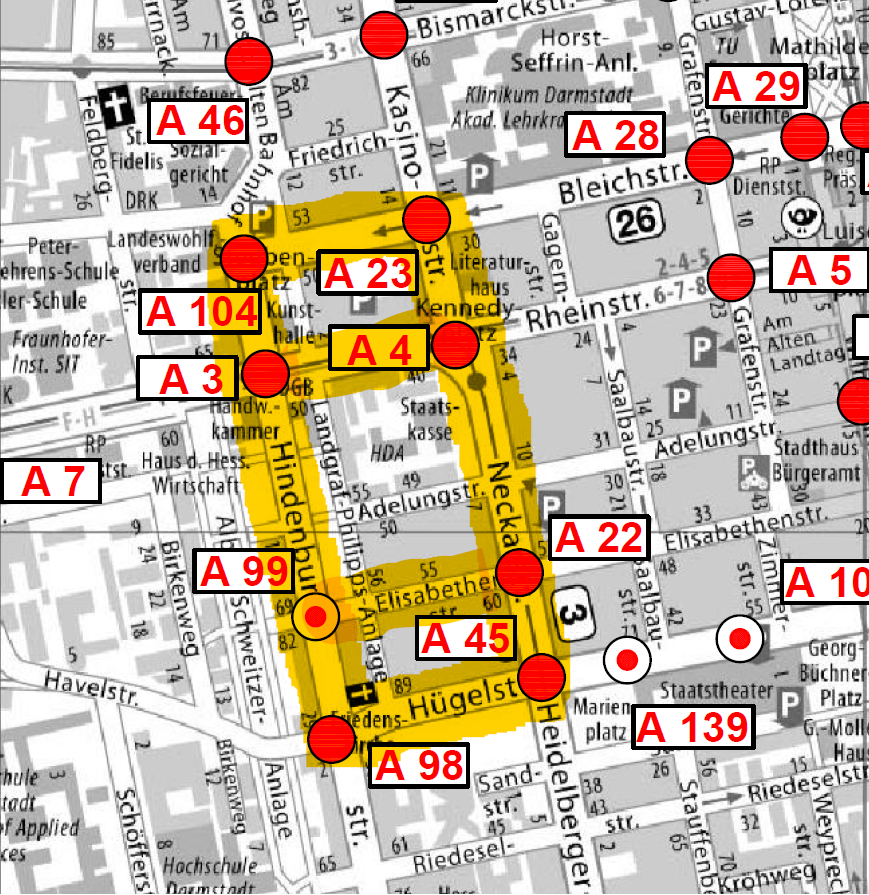
\includegraphics[scale=0.4]{darmstadt.png}
	\caption{Modelowany fragment miasta wraz z punktami pomiarowymi}
	\label{fig:darmstadt}
\end{figure}

\begin{figure}[!htb]
    \centering
    \captionsetup{justification=centering}
   \begin{minipage}{0.48\textwidth}
     \centering
     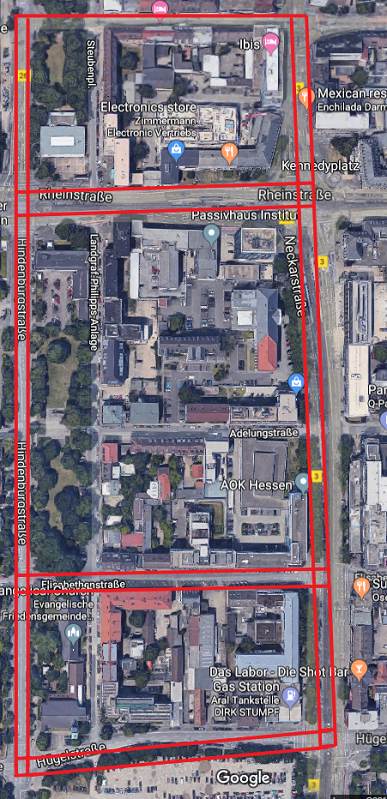
\includegraphics[width=.6\linewidth]{marked_map.png}
     \caption{Rzeczywista mapa obszaru z zaznaczonymi drogami}\label{fig:marked_map}
   \end{minipage}\hfill
   \begin{minipage}{0.48\textwidth}
     \centering
     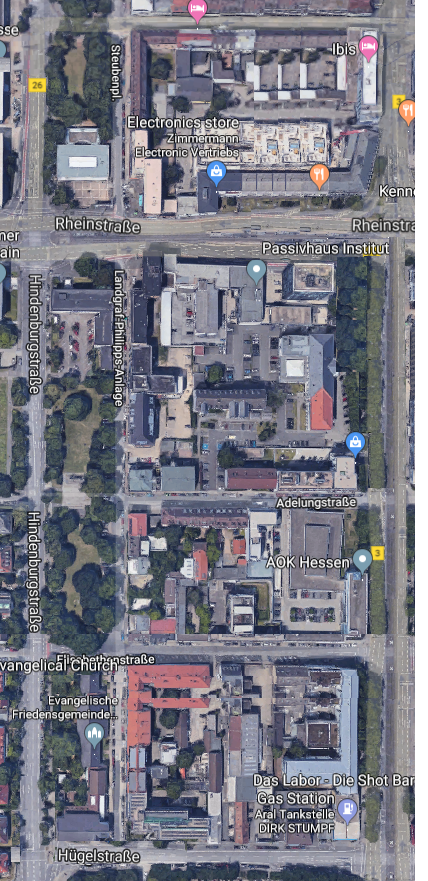
\includegraphics[width=.6\linewidth]{mapa.png}
     \caption{Wyrównana mapa rozpatrywanego obszaru}\label{fig:mapa}
   \end{minipage}
\end{figure}
\newpage
\subsection*{Implementacja modelu}
Model opisany w sekcji \ref{sec:model} został zaimplementowany w języku Python. Taki wybór języka programowania został podyktowany prostotą języka, dużą dostępnością różnorakich bibliotek i narzędzi co pozwoliło na skupienie się na stworzeniu jak najlepszego modelu opisującego badane zjawisko bez znaczących trudności w warstwie implementacyjnej.

Jedyną zewnętrzną biblioteką, niewchodzącą w standard języka, jest biblioteka Matplotlib\footnote{https://matplotlib.org/} która dostarcza narzędzi do tworzenia animowanych wykresów.

Strukturę zaimplementowanego modelu przedstawia diagram klas UML (rysunek \ref{fig:klasy}). Kod źródłowy znajduje się w załączniku do niniejszej dokumentacji.

\begin{figure}[!ht]
	\centering
	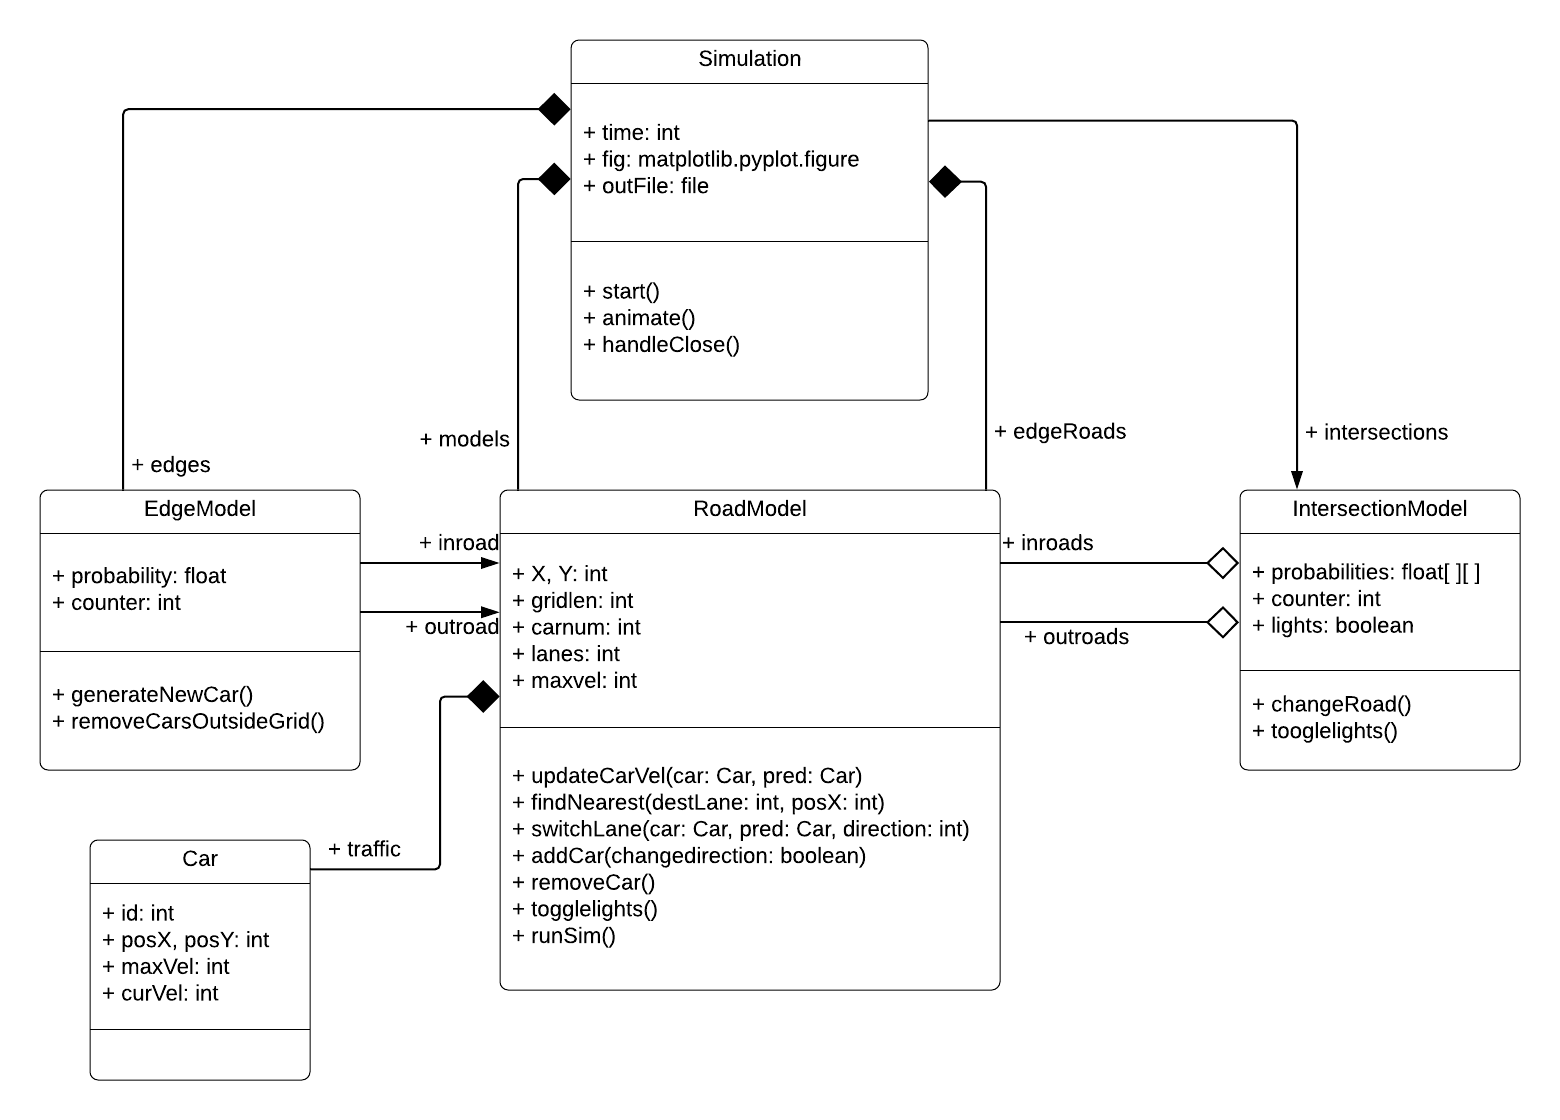
\includegraphics[scale=0.6]{MiSS_Class_Diagram.png}
	\caption{Diagram klas UML}
	\label{fig:klasy}
\end{figure}

\newpage
Przebieg symulacji zaobserwować można na diagramie sekwencji UML (rysunek \ref{fig:sekwencja}).

\begin{figure}[!h]
	\centering
	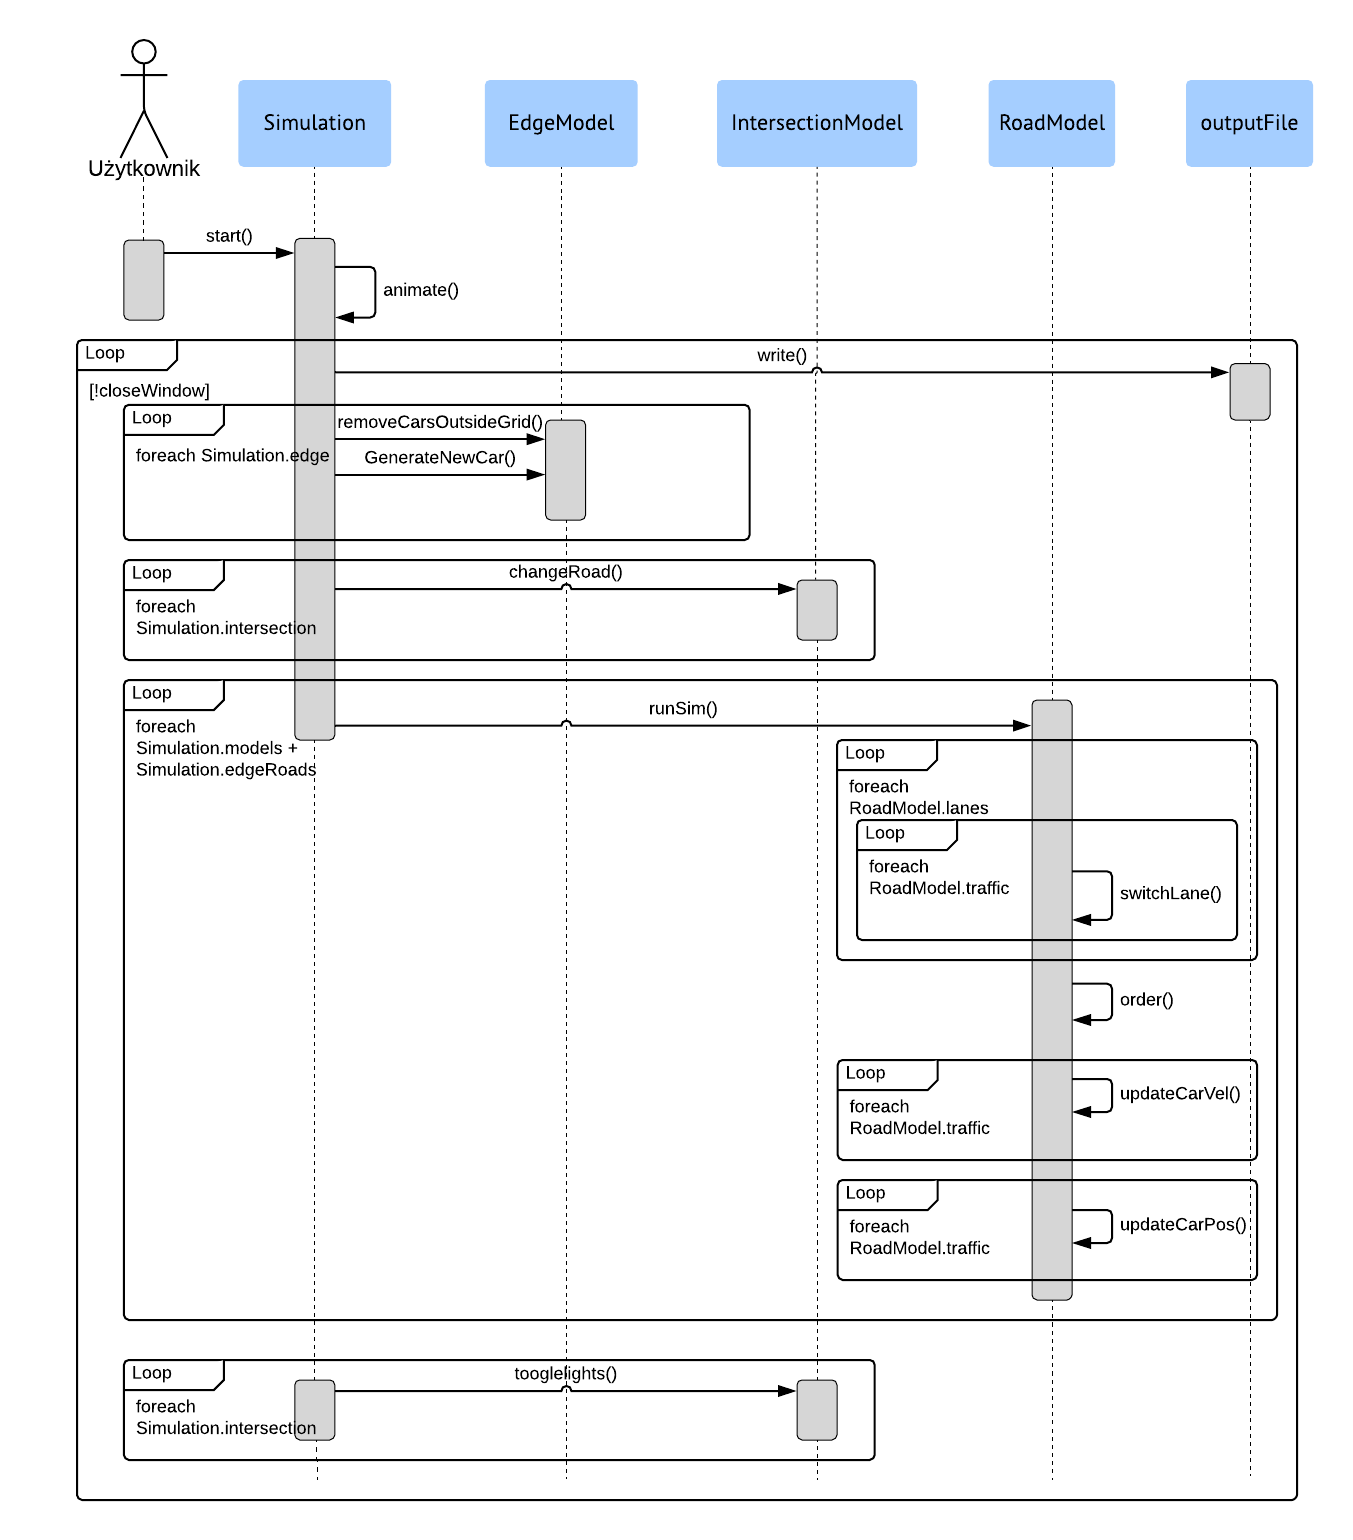
\includegraphics[scale=0.6]{MiSS_Sequene_Diagram.png}
	\caption{Diagram sekwencji UML}
	\label{fig:sekwencja}
\end{figure}

Wejściem prezentowanego przez nas modelu są dane pomiarowe z czujników znajdujących się bezpośrednio wokół badanego obszaru. Stanowią one podstawę do określenia liczby generowanych samochodów które będą się poruszały po ulicach. Po każdej minucie symulacji do pliku wynikowego zapisywane są dane na temat liczby samochodów które pokonały każde z symulowanych skrzyżowań (dane z ,,wirtualnych czujników'' wewnątrz symulacji). 

\subsection*{Przeprowadzane symulacje}
Pierwszym eksperymentem przeprowadzonym w toku symulacji jest zbadanie rozkładu ruchu miejskiego generowanego na podstawie danych wejściowych do modelu. Po przeprowadzeniu symulacji dane wyjściowe z modelu zostaną porównane z odczytami z rzeczywistych czujników na odpowiadających skrzyżowaniach. Eksperyment ten pozwoli na określenie stopnia wiarygodności proponowanego modelu i jego parametrów. 

Drugim eksperymentem będzie sprawdzenie odporności modelu badanego fragmentu sieci miejskiej na znacznie większe natężenie ruchu (w tym przypadku pięciokrotnie większe). Nie jest możliwe porównanie symulacji z rzeczywistością z powodu braku realnych danych w sytuacji pięciokrotnego zwiększenia natężenia ruchu zatem wyniki symulacji oceniane będą jakościowo, analizie podlegać będą powstające zatory, ich rozkład na przestrzeni analizowanego obszaru oraz ogólna płynność ruchu.

\newpage
\section{Wyniki symulacji}
\subsection*{Eksperyment pierwszy}
Wyniki pomiarów z wyjścia modelu w pięciu kolejnych symulacjach wraz z wartościami średnimi zebrane są w tabelach \ref{tab:1} - \ref{tab:5}. Porównanie średnich wyników symulacji z wartościami z danych pomiarowych przedstawione są na rysunkach \ref{fig:1m} - \ref{fig:5m}. Wartości 0 dla czujnika A99 mogą być interpretowane wielorako: skrzyżowanie czasowo wyłączone z ruchu, nieaktywny/uszkodzony czujnik itp. Zerowe natężenie ruchu w tym punkcie zostało uwzględnione przy ustalaniu parametrów modelu. Zapis eksperymentu w załączonym pliku eksperyment1.mov.


\begin{table}[!h]
	\centering

\begin{tabular}{|l|l|l|l|l|l|l|}
\hline
\multicolumn{7}{|c|}{Minuta 1}                                                                                                                                                                                                                   \\ \hline
\multicolumn{1}{|c|}{Czujnik} & \multicolumn{1}{c|}{Symulacja 1} & \multicolumn{1}{c|}{Symulacja 2} & \multicolumn{1}{c|}{Symulacja 3} & \multicolumn{1}{c|}{Symulacja 4} & \multicolumn{1}{c|}{Symulacja 4} & \multicolumn{1}{c|}{Średnia} \\ \hline
A 98                          & 27                               & 26                               & 20                              & 25                             & 26                             & 25                                     \\ \hline
A 45                          & 17                               & 14                               & 19                              & 16                             & 16                             & 16                                     \\ \hline
A 99                          & 0                                & 0                                & 0                               & 0                              & 0                              & 0                                      \\ \hline
A 22                          & 18                               & 20                               & 21                              & 18                             & 17                             & 19                                     \\ \hline
A 3                           & 41                               & 41                               & 43                              & 39                             & 43                             & 41                                     \\ \hline
A 4                           & 35                               & 30                               & 20                              & 31                             & 30                             & 29                                     \\ \hline
A 104                         & 16                               & 10                               & 13                              & 11                             & 17                             & 13                                     \\ \hline
A 23                          & 22                               & 23                               & 15                              & 31                             & 31                             & 24                                     \\ \hline

\end{tabular}
\caption{Pierwsza minuta symulacji}
\label{tab:1}
\end{table}

\begin{table}[!h]
	\centering

\begin{tabular}{|l|l|l|l|l|l|l|}
\hline
\multicolumn{7}{|c|}{Minuta 2}                                                                                                                                                                                                                   \\ \hline
\multicolumn{1}{|c|}{Czujnik} & \multicolumn{1}{c|}{Symulacja 1} & \multicolumn{1}{c|}{Symulacja 2} & \multicolumn{1}{c|}{Symulacja 3} & \multicolumn{1}{c|}{Symulacja 4} & \multicolumn{1}{c|}{Symulacja 5} & \multicolumn{1}{c|}{Średnia} \\ \hline
A 98                          & 11                               & 9                                & 13                              & 19                             & 11                             & 13                                     \\ \hline
A 45                          & 34                               & 21                               & 22                              & 31                             & 28                             & 27                                     \\ \hline
A 99                          & 0                                & 0                                & 0                               & 0                              & 0                              & 0                                      \\ \hline
A 22                          & 14                               & 14                               & 11                              & 14                             & 13                             & 13                                     \\ \hline
A 3                           & 23                               & 19                               & 19                              & 21                             & 22                             & 21                                     \\ \hline
A 4                           & 27                               & 29                               & 25                              & 33                             & 27                             & 28                                     \\ \hline
A 104                         & 14                               & 16                               & 19                              & 12                             & 11                             & 14                                     \\ \hline
A 23                          & 29                               & 26                               & 27                              & 23                             & 25                             & 26                                     \\ \hline
\end{tabular}
\caption{Druga minuta symulacji}
\label{tab:2}
\end{table}
\newpage
\begin{table}[!h]
	\centering

\begin{tabular}{|l|l|l|l|l|l|l|}
\hline
\multicolumn{7}{|c|}{Minuta 3}                                                                                                                                                                                                                   \\ \hline
\multicolumn{1}{|c|}{Czujnik} & \multicolumn{1}{c|}{Symulacja 1} & \multicolumn{1}{c|}{Symulacja 2} & \multicolumn{1}{c|}{Symulacja 3} & \multicolumn{1}{c|}{Symulacja 4} & \multicolumn{1}{c|}{Symulacja 5} & \multicolumn{1}{c|}{Średnia} \\ \hline
A 98                          & 15                               & 17                               & 16                              & 23                             & 21                             & 18                                     \\ \hline
A 45                          & 25                               & 20                               & 26                              & 26                             & 18                             & 23                                     \\ \hline
A 99                          & 0                                & 0                                & 0                               & 0                              & 0                              & 0                                      \\ \hline
A 22                          & 12                               & 13                               & 19                              & 15                             & 12                             & 14                                     \\ \hline
A 3                           & 41                               & 38                               & 34                              & 38                             & 39                             & 38                                     \\ \hline
A 4                           & 41                               & 33                               & 43                              & 35                             & 40                             & 38                                     \\ \hline
A 104                         & 13                               & 20                               & 8                               & 17                             & 15                             & 15                                     \\ \hline
A 23                          & 20                               & 20                               & 22                              & 32                             & 27                             & 24                                     \\ \hline
\end{tabular}
\caption{Trzecia minuta symulacji}
\label{tab:3}
\end{table}

\begin{table}[!h]
	\centering

\begin{tabular}{|l|l|l|l|l|l|l|}
\hline
\multicolumn{7}{|c|}{Minuta 4}                                                                                                                                                                                                                   \\ \hline
\multicolumn{1}{|c|}{Czujnik} & \multicolumn{1}{c|}{Symulacja 1} & \multicolumn{1}{c|}{Symulacja 2} & \multicolumn{1}{c|}{Symulacja 3} & \multicolumn{1}{c|}{Symulacja 4} & \multicolumn{1}{c|}{Symulacja 5} & \multicolumn{1}{c|}{Średnia} \\ \hline
A 98                          & 24                               & 19                               & 26                              & 30                             & 18                             & 23                                     \\ \hline
A 45                          & 25                               & 14                               & 20                              & 26                             & 22                             & 21                                     \\ \hline
A 99                          & 0                                & 0                                & 0                               & 0                              & 0                              & 0                                      \\ \hline
A 22                          & 16                               & 7                                & 17                              & 17                             & 15                             & 14                                     \\ \hline
A 3                           & 44                               & 30                               & 29                              & 29                             & 44                             & 35                                     \\ \hline
A 4                           & 35                               & 31                               & 34                              & 34                             & 42                             & 35                                     \\ \hline
A 104                         & 30                               & 20                               & 34                              & 25                             & 23                             & 26                                     \\ \hline
A 23                          & 33                               & 32                               & 22                              & 26                             & 34                             & 29                                     \\ \hline
\end{tabular}
\caption{Czwarta minuta symulacji}
\label{tab:4}
\end{table}
%\newpage
\begin{table}[!h]
	\centering

\begin{tabular}{|l|l|l|l|l|l|l|}
\hline
\multicolumn{7}{|c|}{Minuta 5}                                                                                                                                                                                                                   \\ \hline
\multicolumn{1}{|c|}{Czujnik} & \multicolumn{1}{c|}{Symulacja 1} & \multicolumn{1}{c|}{Symulacja 2} & \multicolumn{1}{c|}{Symulacja 3} & \multicolumn{1}{c|}{Symulacja 4} & \multicolumn{1}{c|}{Symulacja 5} & \multicolumn{1}{c|}{Średnia} \\ \hline
A 98                          & 15                               & 12                               & 16                              & 12                             & 10                             & 13                                     \\ \hline
A 45                          & 30                               & 14                               & 27                              & 22                             & 20                             & 23                                     \\ \hline
A 99                          & 0                                & 0                                & 0                               & 0                              & 0                              & 0                                      \\ \hline
A 22                          & 22                               & 11                               & 13                              & 12                             & 11                             & 14                                     \\ \hline
A 3                           & 23                               & 28                               & 43                              & 32                             & 22                             & 30                                     \\ \hline
A 4                           & 42                               & 30                               & 41                              & 24                             & 40                             & 35                                     \\ \hline
A 104                         & 16                               & 19                               & 16                              & 12                             & 18                             & 16                                     \\ \hline
A 23                          & 29                               & 36                               & 26                              & 23                             & 33                             & 29                                     \\ \hline
\end{tabular}
\caption{piąta minuta symulacji}
\label{tab:5}
\end{table}
\newpage
\begin{figure}[!h]
    \centering
    \begin{minipage}{0.5\textwidth}
        \centering
        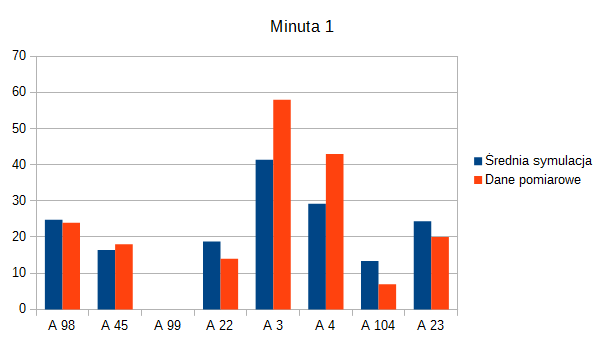
\includegraphics[width=\textwidth]{min1.png} % first figure itself
        \caption{pierwsza minuta symulacji}
        \label{fig:1m}
    \end{minipage}\hfill
    \begin{minipage}{0.5\textwidth}
        \centering
        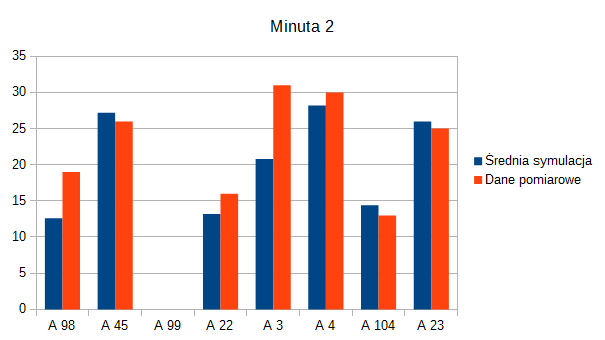
\includegraphics[width=\textwidth]{min2.png} % second figure itself
        \caption{druga minuta symulacji}
        \label{fig:2m}
    \end{minipage}
\end{figure}

\begin{figure}[!ht]
    \centering
    \begin{minipage}{0.5\textwidth}
        \centering
        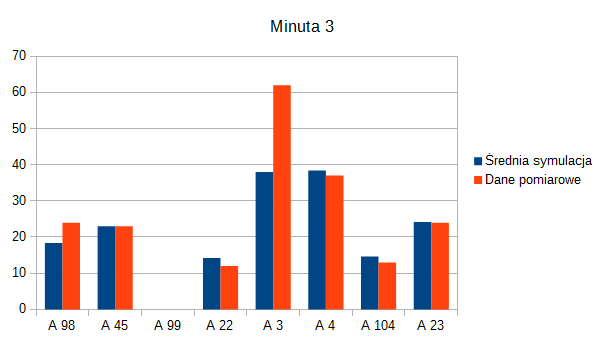
\includegraphics[width=\textwidth]{min3.png} % first figure itself
        \caption{trzecia minuta symulacji}
        \label{fig:3m}
    \end{minipage}\hfill
    \begin{minipage}{0.5\textwidth}
        \centering
        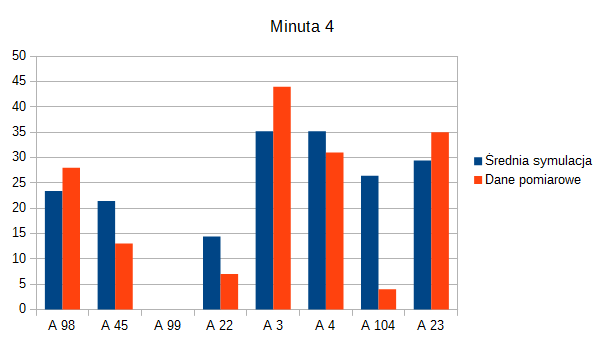
\includegraphics[width=\textwidth]{min4.png} % second figure itself
        \caption{czwarta minuta symulacji}
        \label{fig:4m}
    \end{minipage}
\end{figure}

\begin{figure}[!ht]
    \centering
    \begin{minipage}{0.5\textwidth}
        \centering
        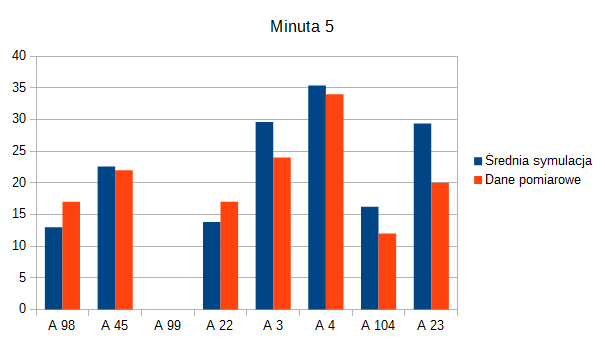
\includegraphics[width=\textwidth]{min5.png} % first figure itself
        \caption{piąta minuta symulacji}
        \label{fig:5m}
    \end{minipage}\hfill
\end{figure}

%\newpage
\subsection*{Eksperyment drugi}
Wyniki drugiego eksperymentu widoczne są w załączonym pliku eksperyment2.mov.

\newpage
%\clearpage
\section{Wnioski}
%\lipsum[2]
Pierwszy z przeprowadzonych eksperymentów pokazuje że zaproponowany model, oraz jego parametry dobrze opisują analizowany obszar. Punktowe rozbieżności między wynikami symulacji oraz danymi rzeczywistymi mogą być wynikiem różnorakich, trudnych do przewidzenia i zamodelowania, czynników (jak na przykład zablokowana droga z powodu dostawy do, stłuczka, przejazd kolumny rządowej itp.). Warto zauważyć, że nie zachodzi zjawisko zwiększenia rozbieżności między danymi z symulacji a danymi pomiarowymi wraz z upływem czasu co potwierdza wiarygodność modelu.

Drugi eksperyment pozwala na ocenę zdolności istniejącej infrastruktury drogowej do przyjęcia znacząco większej liczby samochodów. Jak widać w załączonym zapisie symulacji pięciokrotne zwiększenie natężenia ruchu względem poziomu normalnie występującego powoduje powstawanie znacznych zatorów w obrębie najbardziej uczęszczanych dróg. Jest to często spotykane zjawisko, a zapobieganie mu jest dużym wyzwaniem dla projektantów infrastruktury drogowej. Zauważalne jest również ciekawe zjawisko kompletnego zatorowania ulicy Rheinstraße będącej jedną z głownych arterii miasta, kiedy równolegle do niej znajdują się niemal puste drogi mogące rozładować korek. Zjawisko pokazuje, że modelowanie ruchu miejskiego przedstawione w projekcie ma duży potencjał dla bardzo pożądanego w dzisiejszych czasach zoptymalizowania ruchu miejskiego przez na przykład inteligentne systemy potrafiące z wyprzedzeniem przewidzieć możliwość zatoru i zapobiec jego utworzeniu przez odpowiednie sterowanie sygnalizacją świetlną.
	
Dalszym kierunkiem rozwoju projektu jest dodawanie do modelu następnych cech dodających mu realizmu tak aby jak najdokładniej odzwierciedlał rzeczywistość: uwzględnianie warunków atmosferycznych, pory roku, krzywizn dróg wymuszających zmianę prędkości (następującą w różnej mierze dla pojazdów o różnych gabarytach), losowych wydarzeń jak przejazdy pojazdów uprzywilejowanych (ambulans, straż pożarna), stłuczek czy awarii sygnalizacji świetlnej. W następstwie obiecujących wyników symulacji należy w przyszłości również rozbudować model tak aby obejmował zdecydowanie większy obszar niż 8 skrzyżowań i podczas symulacji zwracać uwagę na gęstość pojazdów w poszczególnych podobszarach.

%\end{enumerate}

\newpage

\bibliographystyle{unsrt}
\bibliography{Bibliografia}
\end{document}
